\documentclass[a4paper,12pt]{article}

% Preamble
\usepackage[T2A]{fontenc}
\usepackage[english,russian]{babel}

\usepackage{amsmath}
\usepackage{graphicx}
\usepackage[utf8]{inputenc}
\usepackage{indentfirst}
\usepackage{caption}
\usepackage{tabularx}
\usepackage{textcomp}
\usepackage{upgreek}
\usepackage[figurename=Фиг.]{caption}
\usepackage{wrapfig}
\graphicspath{{images/}}                                   
\newcommand{\hdotsfive}{. . . . .}
%Preamble

\begin{document}

\noindent

\textsection $ $ \textbf{2.} Пусть \figurename\space\ref{fig1} представляет положения Солнца \textit{S}, Земли \textit{T} и Луны \textit{L}, и пусть $\Theta$ есть центр тяжести Земли и Луны. Делаем следующие обозначения:

\begin{table}[h]
    \begin{center}
        \textbf{Обозначения}\\
        \text{} \\
        \text{}
        \begin{tabular}{clrl}
            Масса           & Солнца & \hdotsfive & \textit{S} \\
            \guillemotright & Земли  & \hdotsfive & \textit{T} \\
            \guillemotright & Луны   & \hdotsfive & \textit{L} \\
        \end{tabular}
        \caption{Обозначения}
    \end{center}
\end{table}

Расстояние:
\begin{equation*}
    \textit{S}\Theta = \uprho; \textit{ST} = \uprho_1; \textit{SL} = \uprho_2; \textit{TL} = \textit{r}\\
\end{equation*}

\noindentтогда будет:
\begin{equation}
    \begin{aligned}
        \textit{T}\Theta & = \textit{r}_1 = \frac{\textit{L}}{\textit{T + L}} \cdot \textit{r} \\
        \textit{L}\Theta & = \textit{r}_2 = \frac{\textit{T}}{\textit{T + L}} \textit{r}
        \label{label1}
    \end{aligned}
\end{equation}

Составим теперь выражения ускорений, которые эти тела сообщают друг другу.

\begin{wrapfigure}{i}{0.5\linewidth}
    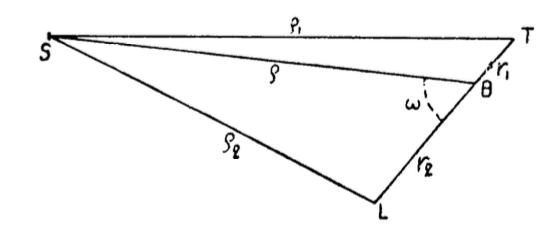
\includegraphics[scale=0.6]{21.png}
    \captionof{figure}{Небесные тела}
\end{wrapfigure}
\label{fig1}

Солнце S сообщает ускорения:
\begin{equation*}
    \begin{aligned}
        \text{Земле: } & f\cdot\frac{\textit{S}}{\uprho_1^2}\text{по направлению}                                   & \textit{TS} \\
        \text{Луне: }  & f\cdot\frac{\textit{S}}{\uprho_2^2}\text{\space\space\guillemotright\space\guillemotright} & \textit{LS}
    \end{aligned}
\end{equation*}
\noindentвследствие чего точка $\Theta$ имеет ускорения:
\\ $ $ \\

\begin{equation*}
    \begin{aligned}
        \frac{T}{T+L} \cdot f \cdot \frac{S}{\uprho_1^2} & \text{по направлению, параллельному}                                         & \textit{TS} \\
        \frac{T}{T+L} \cdot f \cdot \frac{S}{\uprho_2^2} & \text{\space\space\guillemotright\space\guillemotright\space\guillemotright} & \textit{LS}
    \end{aligned}
\end{equation*}

Ускорения Солнца, происходящие от притяжения Земли и Луны, соответственно, суть:

\begin{equation*}
    \begin{aligned}
        f \cdot \frac{T}{\uprho_1^2} & \text{по направлению}                                   & \textit{ST} \\
        f \cdot \frac{T}{\uprho_2^2} & \text{\space\space\guillemotright\space\guillemotright} & \textit{SL} \\
    \end{aligned}
\end{equation*}

\noindentпоэтому ускорения точки $\Theta$ относительно точки S будут:

\begin{equation*}
    \begin{aligned}
        \omega_1 = f \cdot & \frac{(\textit{S + T + L})}{T + L} \cdot \frac{\textit{T}}{\uprho_1^2} & \text{по направлению параллельно}                                            & \textit{TS} \\
        \omega_2 = f \cdot & \frac{\textit{ S + T + L}}{T + L } \cdot \frac{\textit{L}}{\uprho_2^2} & \text{\space\space\guillemotright\space\guillemotright\space\guillemotright} & \textit{LS}
    \end{aligned}
\end{equation*}

Разлагая эти ускорения, соответственно, по направлениям $\Theta$\textit{S} и $\Theta$\textit{L}, получим, как легко видеть из подобия показанных на  \figurename\space\ref{fig2} и \ref{fig3} треугольников:
\begin{equation*}
    \begin{aligned}
        \omega_1 \prime       & = \omega_1 \cdot \frac{\uprho}{\uprho_1} \text{по направлению}                                   & \Theta\textit{S} \\
        \omega_1 \prime\prime & = \omega_1 \cdot \frac{\textit{r}_1}{\uprho_1} \text{\guillemotright\space\guillemotright\space} & \Theta\textit{L} \\
        \omega_2 \prime       & = \omega_2 \cdot \frac{\uprho}{\uprho_2} \text{\guillemotright\space\guillemotright\space}       & \Theta\textit{S} \\
        \omega_2 \prime\prime & = \omega_2 \cdot \frac{\textit{r}_1}{\uprho_2} \text{\guillemotright\space\guillemotright\space} & \textit{L}\Theta
    \end{aligned}
\end{equation*}


\begin{center}
    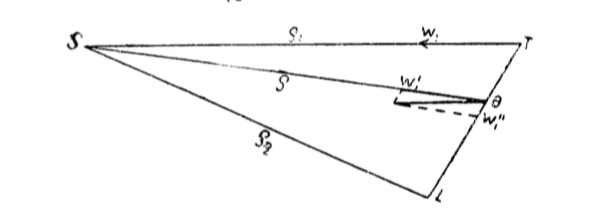
\includegraphics{22.png}
    \captionof{figure}{Расчет ускорений}
    \label{fig2}
\end{center}

\noindentполучим для ускорений точки $\Theta$ слагающие:
\begin{equation*}
    \begin{aligned}
        \textit{W}_1 & =  \omega_1\prime + \omega_2\prime             & = f \cdot & \frac{\textit{S + T + L}}{T + L} \cdot \left[\textit{T} \cdot \frac{\uprho}{\uprho_1^3} + \textit{L} \cdot \frac{\uprho}{\uprho_2^3}\right] & \text{по } \Theta{\textit{S}} \\
        \textit{W}_2 & =  \omega_1\prime\prime - \omega_2\prime\prime & = f \cdot & \frac{\textit{S + T + L}}{T + L} \cdot \left[\textit{T} \cdot \frac{\uprho}{\uprho_1^3} - \textit{L} \cdot \frac{\uprho}{\uprho_2^3}\right] & \text{по } \Theta{\textit{L}}
    \end{aligned}
\end{equation*}

\begin{center}
    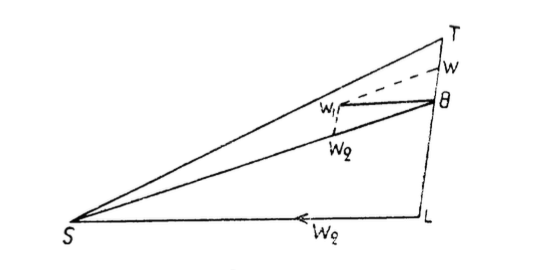
\includegraphics{23.png}
    \captionof{figure}{Результат}
    \label{fig3}
\end{center}

Заменив $r_1$ и $r_2$ выражениями (\ref{label1}), имеем:
\begin{equation*}
    \begin{aligned}
        \textit{W}_1 & = f \cdot \frac{\textit{S + T + L}}{T + L} \cdot \uprho \cdot \left[\frac{\textit{T}}{\uprho_1^3} + \frac{\textit{L}}{\uprho_2^3}\right] \text{по направлению } \Theta{\textit{S}}                      \\
        \textit{W}_2 & = f \cdot \frac{\textit{S + T + L}}{T + L} \cdot \textit{T} \cdot \textit{L} \cdot \textit{r} \cdot \left[\frac{1}{\uprho_1^3} - \frac{1}{\uprho_2^3}\right]  \text{по направлению } \Theta{\textit{L}}
    \end{aligned}
\end{equation*}

\noindentНо

\begin{equation*}
    \begin{aligned}
        \uprho_1^2 & = \uprho^2 + 2\uprho\cdot & \frac{\textit{L}}{\textit{T + L}}\cdot & \textit{r}\cos\omega + \left( \frac{\textit{L}}{\textit{T + L}} \cdot \textit{r} \right)^2 \\
        \uprho_2^2 & = \uprho^2 - 2\uprho      & \frac{\textit{T}}{\textit{T + L}}      & \textit{r}\cos\omega + \left( \frac{\textit{L}}{\textit{T + L}} \textit{r} \right)^2
    \end{aligned}
\end{equation*}

\noindentследовательно:

\begin{equation*}
    \begin{aligned}
        \frac{1}{\uprho_1^3} = \frac{1}{\uprho^3}\left[ 1 + 3\frac{\textit{L}}{\textit{T+L}}\cos\omega + \left(\frac{\textit{L}}{\textit{T + L}}\textit{r}\right)^2\left(-\frac{3}{2} + \frac{15}{2}\cos^2\omega\right)+ ...\right] \\
        \frac{1}{\uprho_2^3} = \frac{1}{\uprho^3}\left[ 1 + 3\frac{\textit{T}}{\textit{T+L}}\cos\omega + \left(\frac{\textit{L}}{\textit{T + L}}\textit{r}\right)^2\left(-\frac{3}{2} + \frac{15}{2}\cos^2\omega\right)+ ...\right]
    \end{aligned}
\end{equation*}

\noindentПодставляя эти выражения, имеем:

\begin{equation*}
    \begin{aligned}
        \textit{W}_1 & = f \cdot \frac{\textit{S + T + L}}{\uprho^2} \left[1 + \frac{\textit{T}\cdot\textit{L}}{(\textit{T + L})^2} \cdot \frac{\textit{r}^2}{\uprho^2}\left(-\frac{3}{2} + \frac{15}{2} \cos^2\omega\right) + ...\right] \\
        \textit{W}_2 & = f \cdot \frac{\textit{S + T + L}}{\uprho^2} \left[-3 \cdot \frac{\textit{T}\cdot\textit{L}}{(\textit{T + L})^2} \cdot \frac{\textit{r}^2}{\uprho^2}\cos\omega + ...\right]
    \end{aligned}
\end{equation*}

\noindentНо отношения

\begin{equation*}
    \begin{aligned}
        \frac{\textit{L}}{\textit{T + L}} \approx \frac{1}{80}; \frac{\textit{r}}{\uprho} \approx \frac{1}{400}; \left(\frac{\textit{r}}{\uprho}\right)^2 \approx \frac{1}{160000}
    \end{aligned}
\end{equation*}

\noindentпоэтому будет

\begin{equation*}
    \begin{aligned}
        \frac{\textit{T} \cdot \textit{L}}{(\textit{T + L})^2} \cdot \frac{r^2}{\uprho^2} \approx \frac{1}{12800000}
    \end{aligned}
\end{equation*}

\noindentи члены, содержащие этот множитель, могут быть отброшены, так что будет:

\begin{equation*}
    \begin{aligned}
        \textit{W}_1 & = f \cdot \frac{\textit{S + T + L}}{\uprho^2} \text{ по направлению } \Theta{\textit{S}} \\
        \textit{W}_2 & = 0 \text{ по направлению } \Theta{\textit{L}}
    \end{aligned}
\end{equation*}

Отсюда следует, что точка $\Theta$ движется вокруг Солнца по эллиптической орбите по законам Кеплера.

Рассмотрим теперь ускорение Луны по отношению к Земле, для чего к ускорениям, сообщаемым Луне Солнцем и Землею, надо присовокупить ускорение, равное и противоположное ускорению земли, происходящему от действия Солнца и Луны. Поступив подобно предыдущему, получим:

\begin{equation*}
    \begin{aligned}
        f \cdot \frac{\textit{T + L}}{\textit{r}^2} + f \cdot \textit{S} \left[\frac{\textit{r}_2}{\uprho_2^3} + \frac{\textit{r}_1}{\uprho_1^3}\right] \text{по направлению } {\textit{L}}\Theta \\
        f \cdot \textit{S} \cdot \uprho \cdot \left[\frac{1}{\uprho_1^3} - \frac{1}{\uprho_2^3}\right]  \text{параллельно } \Theta{\textit{S}}
    \end{aligned}
\end{equation*}

\noindentположим:

\begin{equation*}
    \begin{aligned}
        \textit{T + L} = \mu; \textit{S} = \textit{M}
    \end{aligned}
\end{equation*}

\listoffigures
\listoftables

\end{document}